\documentclass[letter]{article}
\usepackage{amsmath}
\usepackage{amsfonts}
\usepackage{amssymb}
\usepackage{ifthen}
\usepackage{fancyhdr}
\usepackage{graphicx}
\usepackage{caption}
\usepackage{subcaption}
\usepackage{tikz}
\usetikzlibrary{shapes.geometric, arrows}

\tikzstyle{startstop} = [rectangle, rounded corners, minimum width=3cm, minimum height=1cm,text centered, draw=black, fill=red!30]
\tikzstyle{process} = [rectangle, minimum width=3cm, minimum height=1cm, text centered, draw=black, fill=blue!30]
\tikzstyle{decision} = [diamond, minimum width=3cm, minimum height=1cm, text centered, draw=black, fill=green!30, aspect=2]
\tikzstyle{arrow} = [thick,->,>=stealth]
\usepackage{subcaption}
\usepackage[backend=biber]{biblatex}
\addbibresource{references.bib}


%%%
% Set up the margins to use a fairly large area of the page
%%%
\oddsidemargin=.2in
\evensidemargin=.2in
\textwidth=6in
\topmargin=0in
\textheight=9.0in
\parskip=.07in
\parindent=0in
\pagestyle{fancy}

%%%
% Set up the header
%%%
\newcommand{\setheader}[6]{
	\lhead{{\sc #1}\\{\sc #2} } %% ({\small \it \today}) for date on the top left
	\rhead{
		{\bf #3} 
		\ifthenelse{\equal{#4}{}}{}{(#4)}\\
		{\bf #5} 
		\ifthenelse{\equal{#6}{}}{}{(#6)}%
	}
}



%%%
% This is where the body of the document goes
%%%
\begin{document}
\begin{titlepage}
    \begin{center}
        \vspace*{1cm}
 
        \Huge\textbf{Associations Between Tumour Characteristics and Tumour Size in Early Breast Cancer Patients}
 
        \vspace{0.5cm}
        \huge  A Regression Approach
             
        \vspace{1.5cm}
 
        \Large \textbf{Brian Xue, Sami Ahmed, Nzube Ogbu, Matthew Inkim, Cyrus Chung}

        \begin{abstract}
        Breast cancer prognosis and treatment decisions often depend on tumour size, which reflects both intrinsic tumour biology and patient-specific factors. This study investigates whether tumour size in Early Breast Cancer (EBC) patients with clinically negative axillary lymph nodes can be explained by age, number of lymph node metastases, Ki67 index, estrogen receptor (ER), 
        progesterone receptor (PR), human epidermal growth factor receptor 2 (HER2) status, tumour type, and molecular subtype. Using a multiple linear regression framework with square-root transformation of tumour size to stabilize variance, we evaluated the contribution of each factor while adjusting for the others. The final model revealed a significant positive association between Ki67 and tumour size, 
        supporting its role as a proliferation biomarker. Lymph node metastases were also strongly associated with larger tumours, while ER, PR, and HER2 effects were less pronounced but consistent with established tumour biology. Although the model provided interpretable estimates, limitations included underrepresentation of some tumour subtypes, potential omitted variable bias, receptor status discordance, 
        and the assumption of linear additive effects. These findings reinforce the biological relevance of Ki67 and lymph node involvement in tumour growth, while highlighting the need for models that capture non-linear and interactive effects in breast cancer progression.

        \end{abstract}
 
        \vfill
             
        STA302: Methods of Data Analysis I\\
        Larry Dong\\
        August 15, 2025
             
        \vspace{0.8cm}
             
        Department of Statistical Sciences\\
        University of Toronto\\
    
    \end{center}

\newpage

\tableofcontents

\newpage

\end{titlepage}

\setheader{STA302}{Methods of Data Analysis}{B. Xue, S. Ahmed, N.Ogbu, M. Inkim, C. Chang}{}{}{} 


\section{Introduction}

\large Breast cancer is a leading cause of cancer-related mortality worldwide, and understanding factors associated with tumour size is crucial for prognosis, treatment planning, and insights into disease biology. Tumour size can be influenced by tumour-intrinsic features, such as growth rate and molecular characteristics, and patient-specific factors, including age and overall health. 

\textit{This study examines whether tumour size can be described using patient age, number of lymph node metastases, Ki67 index, Estrogen Receptor (ER)/Progesterone Receptor (PR)/Human Epidermal Growth Factor Receptor 2 (HER2) status, tumour type, and molecular subtype in Early Breast Cancer (EBC) patients with clinically negative Axillary Lymph Nodes (ALN).}

\textbf{Hypothesis:} Ki67 is a biomarker used to assess the rate of cell division in cancer cells. We assume that a higher Ki67 value results in larger tumours.

Previous research supports the plausibility of these relationships. \cite{Jones2023} linked cancer cell size to systematic shifts in protein abundance, suggesting size-related molecular signatures. \cite{Fang2011} showed that tumour size influences the concentration of tumour-derived proteins in plasma in a nonlinear manner, indicating that measurable tumour characteristics reflect underlying biological changes. \cite{Li2015} demonstrated that specific circulating proteins increase consistently as tumours grow, highlighting the role of measurable biological markers in tracking tumour progression.

Given that tumour size and the selected predictors are quantitative or categorical variables, linear regression is an appropriate tool to evaluate these relationships. This approach allows for clear interpretation of how each factor is associated with tumour size while adjusting for others, with emphasis on interpretability and description rather than pure prediction.

\newpage

\section{Methods}

\subsection{Methodology Flowchart}

\begin{figure}[h!]
\centering
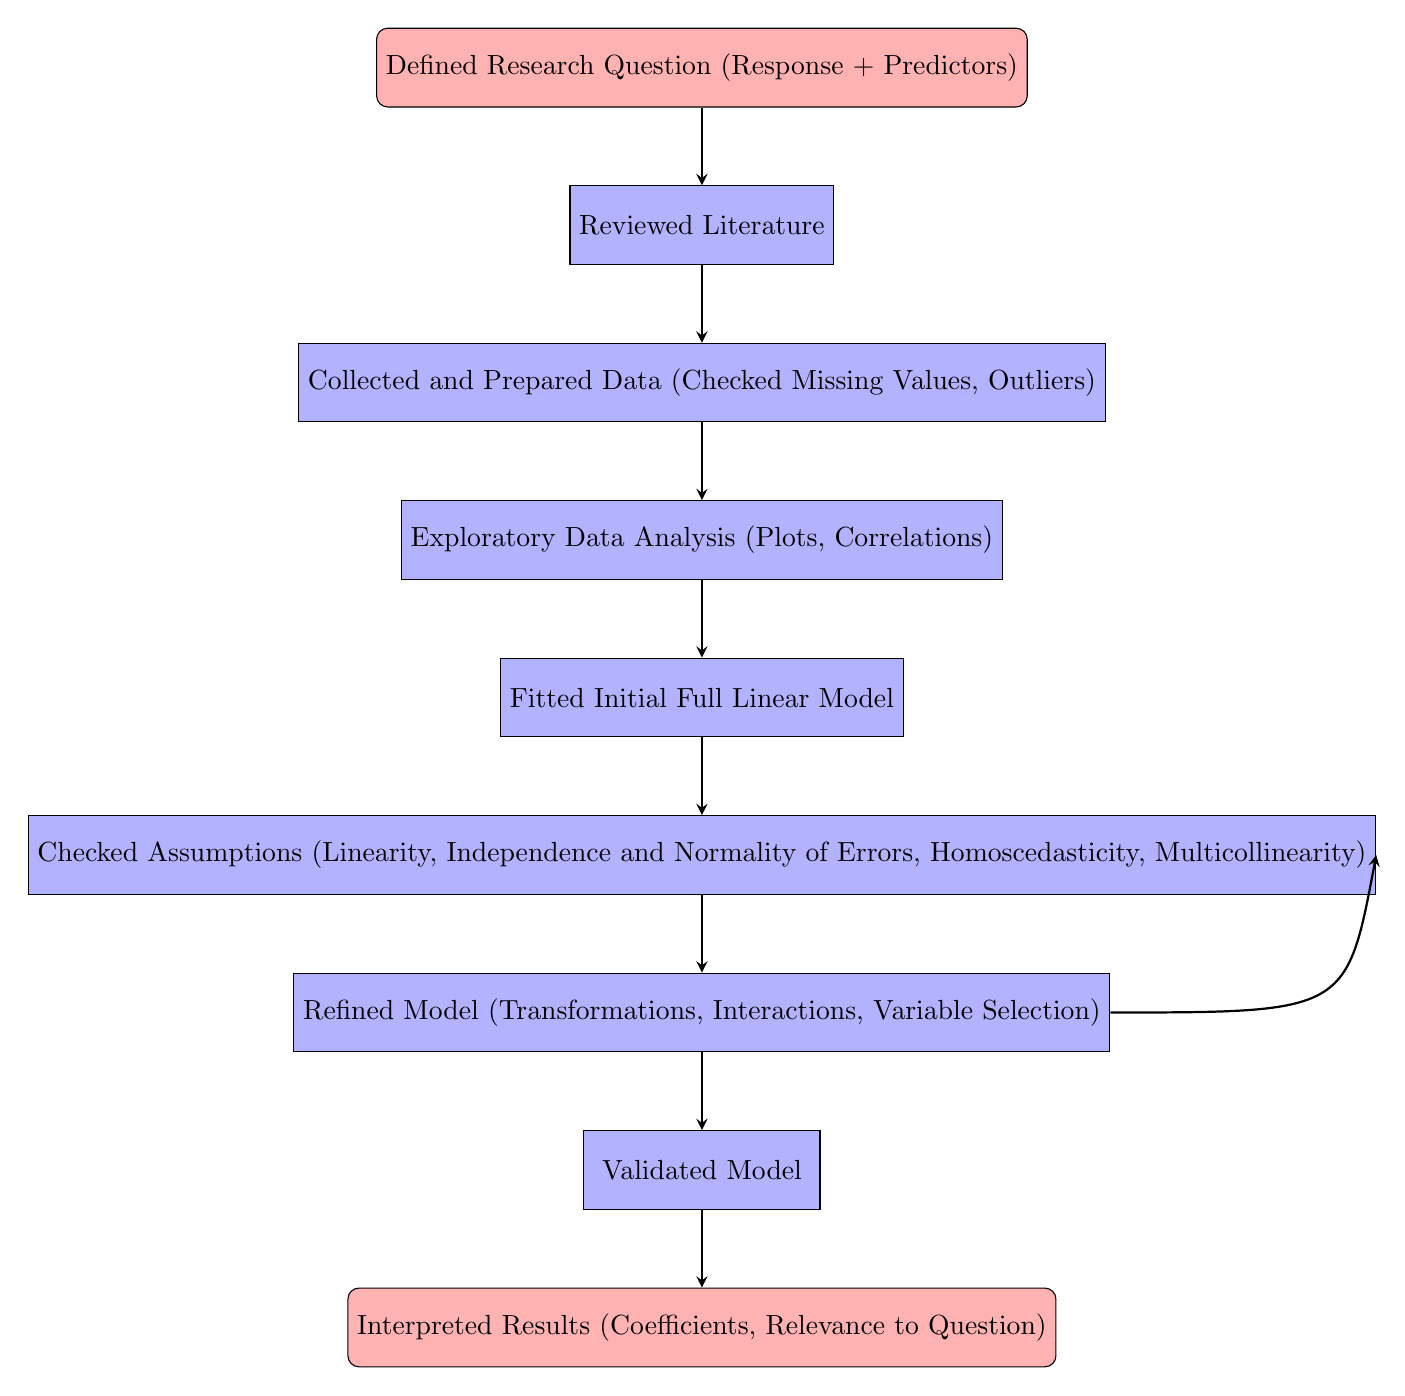
\begin{tikzpicture}[node distance=2cm]

% Nodes (no \\ inside node text)
\node (start) [startstop] {Defined Research Question (Response + Predictors)};
\node (lit) [process, below of=start] {Reviewed Literature };
\node (data) [process, below of=lit] {Collected and Prepared Data (Checked Missing Values, Outliers)};
\node (eda) [process, below of=data] {Exploratory Data Analysis (Plots, Correlations)};
\node (model) [process, below of=eda] {Fitted Initial Full Linear Model};
\node (assump) [process, below of=model] {Checked Assumptions (Linearity, Independence and Normality of Errors, Homoscedasticity, Multicollinearity)};
\node (refine) [process, below of=assump] {Refined Model (Transformations, Interactions, Variable Selection)};
\node (validate) [process, below of=refine] {Validated Model};
\node (interpret) [startstop, below of=validate] {Interpreted Results (Coefficients, Relevance to Question)};

% Arrows
\draw [arrow] (start) -- (lit);
\draw [arrow] (lit) -- (data);
\draw [arrow] (data) -- (eda);
\draw [arrow] (eda) -- (model);
\draw [arrow] (model) -- (assump);
\draw [arrow] (assump) -- (refine);
\draw [arrow] (refine) -- (validate);
\draw [arrow] (validate) -- (interpret);
\draw [arrow] (refine.east) .. controls ++(3,0) .. (assump.east);

\end{tikzpicture}
\caption{Flowchart of study methodology}
\end{figure}

\newpage

\subsection{Data Preparation and Exploratory Analysis}

Data was obtained from the “Early Breast Cancer Core-Needle Biopsy WSI Dataset” \cite{Zhu2021} used in \cite{Xu2021}, which developed a deep learning-based primary tumour biopsy 
signature to predict ALN metastases in EBC patients with clinically negative ALN. After exclusions, 1058 patients were analyzed.

We treated tumour size (cm) as a continuous response variable, while predictors included both continuous (age, Ki67, number of metastases (META))
and categorical variables (ER/PR/HER2/, tumour type (TT), molecular subtype (MST)).

Continuous predictors were assessed for missing values, distributional characteristics, and outliers. Summary statistics and visualisations 
(scatterplots for continuous variables, and boxplots for categorical predictors) were used to assess initial associations with tumour size.
Pearson correlations and one-way ANOVAs were used to preliminarily explore relationships between predictors and response. 

Skewness was examined for continuous variables to detect deviations from normality, and correlations between predictors was assessed to anticipate multicollinearity in the model.

\subsection{Initial Model Specification}

An initial multiple linear regression (MLR) model fit and included all the predictors. This served as the baseline for diagnostics  and refinement.
The focus was on interpretability to determine the independent contribution of each predictor, particularly Ki67, to tumour size. Giving:

\[Y_{\sqrt\text{tumour size}} = \beta_{\text{META}}x_1 + \beta_{\text{age}}x_2 + \beta_{\text{Ki67}}x_3 + \beta_{\text{ER}}x_4 + \beta_{\text{PR}}x_5 + \beta_{\text{HER2}}x_6 
+ \beta_{\text{TT}}x_6 + \beta_{\text{MST}}x_7 + \epsilon \]

Dummy variables were used for categorical variables, and reference levels were chosen based on relevance to ensure interpretable coefficients. 
Continuous predictors were centered to facilitate interpretation of the intercept and reduce potential multicollinearity.
\subsection{Assumption Checks}

The standard regression assumptions were then evaluated. We looked at residuals versus fitted plots for linearity, scale-location plots for homoscedasticity, Q-Q plots for normality,
and Variance Inflation Factor (VIF) for multicollinearity. If assumptions were violated, appropriate mitigation strategies were implemented, including polynomial terms for non-linear trends,
 and centering or standardizing predictors. %Box–Cox or log transformations of the response,

\subsection{Outliers and Influential Observations}

Outlier and influence diagnostics were conducted using Cook's Distance, leverage and DFBETAs. Potential outliers were flagged but not immediately removed, instead kept for further review.
The criteria for being flagged were $leverage > \frac{2p}{n}$, cooks distance > 1, and DFBETA > 1. Graphical representations and influence plots were used to visualise these points.

\subsection{Model Refinement}

As stated above, transformations of the response and/or predictors were aplied when assumption violations were detected. Interaction terms(Ki67 x MST, ER x PR etc.), and polynomial terms were explored when suggested by
residual patterns. Model refinement was guided by statistical criteria and clinical rationale; nested models were compared using ANOVA F-tests, and non-nested models were evaluated with AIC and BIC to identify the ``best" model.
This process was iterative, with assumption checks repeated after each modification to ensure the final model satisfied linear regression requirements.


\subsection{Validation}

The final model was assessed on whether all assumptions were met, the amount of high-influence points was reasonable, $VIF \leq 5$, interpretability, and metrics such as $R^2$ and standardised residuals.

\subsection{Interpretation}

Final model coefficients and confidence intervals were interpreted to determine the independent effects of each predictor on tumour size. Particular attention was given to Ki67 as a biomarker of cell proliferation. 
The clinical relevance of the coefficients was considered, and potential limitations, including sample size, measurement error, and generalizability to other populations, were discussed when drawing conclusions.

\newpage

\section{Results}

The response variable in this model is the diameter of tumours. Initially,
the tumour size exhibited a mean of 2.235 cm, a standard deviation of 0.863 cm, and a minimum
of 0.5 cm, suggesting a right-skewed distribution.

Since MLR assumes that the
residuals of the response variable are normally distributed, this skewness raises concerns about
the model. A square root transformation (SRTS) was applied to the tumour size , resulting in a
more symmetrical distribution with a reduced mean of 1.467 and a standard deviation of 0.290.
SRTS is continuous, unbounded, and approximately normal after transformation.
Hence, suitable for MLR.

\begin{figure}[hbt!]
        \centering
        \includegraphics[width=\textwidth]{sqrt_Diagnostics.png}
        \caption{(a) Residuals versus fitted (b) Q-Q Residuals (c) Scale-Location (d) Residuals versus leverage - The diagnostic plots after the transformation}
\end{figure}

The initial residuals vs. fitted plot showed a downward trend, indicating missing non-linear effects. Applying SRTS produced a more random scatter around zero.
Although a faint trend remains, it reflects dataset characteristics (see section 5.1), so the linearity assumption is reasonably satisfied.

Before transformation, the Q-Q plot showed a faint S-shape with tail deviations, indicating skewed residuals. Applying SRTS stabilized variance and reduced skewness, 
and aligned residuals closer to the 45° line, thereby satisfying the normality assumption and supporting valid inference in the linear regression model.

The scale-location plot of the initial model (see appendix Figure 5) shows even variance of standardized residuals across fitted values, although obvious parabolic patterns are visible. These curves suggest that
certain subsets of observations share similar fitted values and residual spreads, which may occur when categorical predictors produce grouped patterns in the data. To investigate, scale-location plots were 
generated with points colored by each categorical predictor (HER2, ER, PR, Tumour Type, and Molecular Subtype; Figure 3). 



\begin{figure}[htbp]
\centering

% --- Top row: 3 images ---
\begin{subfigure}[b]{0.32\textwidth}
    \includegraphics[width=\textwidth]{Color1.png}
    
\end{subfigure}
\hfill
\begin{subfigure}[b]{0.32\textwidth}
    \includegraphics[width=\textwidth]{Color2.png}
    %\caption{Plot 2}
\end{subfigure}
\hfill
\begin{subfigure}[b]{0.32\textwidth}
    \includegraphics[width=\textwidth]{Color3.png}
    %\caption{Plot 3}
\end{subfigure}

\vspace{0.5cm}

% --- Bottom row: 2 images ---
\begin{subfigure}[b]{0.48\textwidth}
    \includegraphics[width=\textwidth]{Color4.png}
    %\caption{Plot 4}
\end{subfigure}
\hfill
\begin{subfigure}[b]{0.48\textwidth}
    \includegraphics[width=\textwidth]{Color5.png}
    %\caption{Plot 5}
\end{subfigure}

\caption{Colour Coded Scale-Location Plots, filtered by HER2, ER, PR, TT, and MST}
\label{fig:combined_plots}
\end{figure}

In the coloured plots, no category displayed a systematic deviation from the horizontal trend line, and the variance appeared comparable across levels. The observed parabolas were roughly symmetric in the sense 
that if the plots were flipped horizontally, the residual distribution would appear similar, indicating no directional heteroscedasticity related to fitted values.

Given that neither the original nor the color-coded plots reveal substantial issues, the homoscedasticity assumption is considered to be reasonably met. 
The structured patterns are likely due to hidden predictors or some interaction terms that are not available in the dataset, rather than violations caused by included variables.

There are 74 observations with high leverage. However, there are 0 observations with a DFBETA greater than the threshold of 1, nor are there any observations with a Cook's Distance exceeding 1. This would suggest that any existing leverage point is a ``good leverage point", not likely to influence the model, negatively or otherwise. Thus, we can safely assume an absence of outliers, per the decided upon criteria. 
 (see appendix figure 6)


\begin{table}[htbp]
\centering
\label{tab:anova_results}
\begin{tabular}{lrrrr}
\hline
\textbf{Predictor} & \textbf{Sum Sq} & \textbf{Df} & \textbf{$F$ value} & \textbf{$\Pr(>F)$} \\
\hline
\multicolumn{5}{l}{\textit{Type II ANOVA}} \\
Age (years)                       & 0.292 & 1 & 3.8386 & 0.0504\textsuperscript{.} \\
Ki67                               & 0.825 & 1 & 10.8372 & 0.0010\textsuperscript{**} \\
ER                                 & 0.003 & 1 & 0.0401 & 0.8413 \\
PR                                 & 0.361 & 1 & 4.7414 & 0.0297\textsuperscript{*} \\
HER2                               & 0.000 & 1 & 0.0003 & 0.9869 \\
Tumour Type                        & 0.304 & 2 & 1.9952 & 0.1365 \\
Number of lymph node metastases    & 4.986 & 1 & 65.5002 & $1.64\times10^{-15}$\textsuperscript{***} \\
Molecular subtype                  & 0.025 & 3 & 0.1107 & 0.9539 \\
Residuals                          & 78.019 & 1025 &  &  \\
\hline
\multicolumn{5}{l}{\textit{Type III ANOVA}} \\
(Intercept)                        & 6.484 & 1 & 85.1907 & $< 2.2\times10^{-16}$\textsuperscript{***} \\
Age (years)                        & 0.292 & 1 & 3.8386 & 0.0504\textsuperscript{.} \\
Ki67                                & 0.825 & 1 & 10.8372 & 0.0010\textsuperscript{**} \\
ER                                  & 0.003 & 1 & 0.0401 & 0.8413 \\
PR                                  & 0.361 & 1 & 4.7414 & 0.0297\textsuperscript{*} \\
HER2                                & 0.000 & 1 & 0.0003 & 0.9869 \\
Tumour Type                         & 0.304 & 2 & 1.9952 & 0.1365 \\
Number of lymph node metastases     & 4.986 & 1 & 65.5002 & $1.64\times10^{-15}$\textsuperscript{***} \\
Molecular subtype                   & 0.025 & 3 & 0.1107 & 0.9539 \\
Residuals                           & 78.019 & 1025 &  &  \\
\hline
\end{tabular}
\begin{flushleft}
\textsuperscript{.} $p < 0.1$, \textsuperscript{*} $p < 0.05$, \textsuperscript{**} $p < 0.01$, \textsuperscript{***} $p < 0.001$.
\end{flushleft}
\caption{ANOVA results for the model predicting $\sqrt{\text{Tumour Size (cm)}}$}
\end{table}

\begin{table}[ht]
\centering
\label{tab:vif}
\begin{tabular}{lccc}
\hline
\textbf{Predictor} & \textbf{GVIF} & \textbf{Df} & \textbf{GVIF$^{1/(2 \times \text{Df})}$} \\
\hline
Age (years) & 1.047 & 1 & 1.023 \\
Ki67 & 1.686 & 1 & 1.299 \\
ER & 4.047 & 1 & 2.012 \\
PR & 3.017 & 1 & 1.737 \\
HER2 & 51.214 & 1 & 7.156 \\
Tumour Type & 1.047 & 2 & 1.012 \\
Number of lymph node metastases & 1.020 & 1 & 1.010 \\
Molecular subtype & 166.991 & 3 & 2.347 \\
\hline
\end{tabular}
\caption{Variance Inflation Factor (VIF) for predictors in the tumour size model}
\end{table}

\newpage

The ANOVA (Table 1) and VIF (Table 2) results support a clear understanding of the predictors of tumour size. Ki67, representing the percentage of actively dividing tumour cells, is highly significant 
$(F = 10.84, p = 0.001)$ and exhibits low multicollinearity $(VIF \approx 1.30)$, confirming its independent contribution to tumour size, consistent with the hypothesis that higher proliferation rates produce larger tumours. 

Lymph node metastases, indicating cancer spread to axillary nodes, are the strongest predictor $(F = 65.50, p < 0.001)$ and show minimal multicollinearity $(VIF \approx 1.01)$, aligning with literature demonstrating their correlation with tumour size \cite{Min2021}.
(see appendix figure 7 for comparison between the two)

Age and PR are modestly associated $(F \approx 3.84 \text{ and } 4.74, \quad p \approx 0.05 \text{ and } 0.03)$ and show low VIFs $(<2)$, indicating reliable estimation. 
ER shows no significant effect $(F = 0.04, p = 0.84)$, while HER2 and molecular subtype have high VIFs $(\approx 7.16 \text{ and } 2.35)$, suggesting moderate-to-high collinearity, and tumour type is non-significant $(F = 1.99, p = 0.14)$.

Overall, the model supports that Ki67, and lymph node metastases are key continuous predictors of tumour size, while categorical biomarkers require cautious interpretation due to potential collinearity.

\newpage

Figure 4 illustrates the predicted tumour size across the observed range of Ki67, while holding all other predictors at typical values. The highlighted region represents $\pm 10\%$ increase or decrease in Ki67 and how that translates to a 0.05cm increase or decrease in tumour size respectively.

Tumour size was back-transformed from the square-root scale used in the model to allow straightforward interpretation. 
The graph addresses the research question by illustrating how increases in Ki67 correspond to larger tumours, supporting the hypothesis that higher proliferation rates (higher Ki67) drive tumour growth.


\begin{figure}[hbt!]
        \centering
        \includegraphics[width=\textwidth]{PTS_K.png}
        \caption{Predicted Tumour Size vs Ki67, other predictors held constant}
\end{figure}
\newpage

\section{Conclusion and Limitations}
\subsection{Interpretation of Final Model}

The final linear model demonstrates a significant positive association between Ki67 and predicted tumour size, indicating that higher proliferation rates correspond to larger tumours. 
Predicted tumour size was back-transformed from the square-root scale to maintain interpretability in centimetres, ensuring that model predictions align with observed units. While ER, PR, and HER2 were included as predictors, their effects were less pronounced, 
consistent with prior work showing correlations between receptor status and tumour biology \cite{Kozakiewicz2013}. Including these markers enhances interpretability without dominating the model, 
and captures variations linked to tumour type and size. \cite{Thakar2011}

\subsection{Research Question Discussion}

Interaction effects were not considered, which may obscure combined effects of predictors. Discordance in receptor status \cite{Walter2020} introduces variability, contributing to residual trends. 
Extreme values and underrepresentation of some tumour subtypes reduce generalizability. The model assumes linear additive effects and cannot capture non-linear or complex interactions in tumour biology.

Our model directly addresses the research question by quantifying how Ki67, age, lymph node metastases, tumour type, molecular subtype, and receptor status collectively relate to tumour size. 
The strong effect of lymph node metastases is consistent with literature highlighting their role in tumour burden. Ki67 emerges as a key predictor, supporting its use as a proliferation biomarker. The faint parabolic trend in the scale-location plot may reflect 
partial receptor discordance between primary tumours and metastatic sites \cite{Walter2020}, indicating inherent biological variability rather than model mis-specification.

\subsection{Limitations of Analysis}

Several limitations affect the robustness and generalizability of the model. Interaction effects were not considered, which may obscure combined effects of predictors. Omitted variable bias may arise if other biological or genetic factors influencing tumour size are missing. 
The dataset may not represent the broader population, being limited by geography, age, or clinical characteristics. Multicollinearity among predictors can inflate standard errors and destabilize coefficients. 
Our sample size is relatively small (just above a 1000), and tumour type is skewed toward invasive ductal carcinomas (90.45\%), underrepresenting invasive lobular (2.41\%) and other tumours (7.14\%). 
Linear regression does not account for temporal dynamics as tumour size and predictors are measured at different points.

\newpage

\section{Appendix}

\begin{figure}[hbt!]
        \centering
        \includegraphics[width=\textwidth]{pre_initial.png}
        \caption{(a) Residuals versus fitted (b) Q-Q Residuals (c) Scale-Location (d) Residuals vs leverage - Diagnostic plots before the transformation}
\end{figure}

\begin{figure}[hbt!]
        \centering
        \includegraphics[width=\textwidth]{Leverage_DFBTA.png}
        \caption{(a and b) Leverage and Leverage Histogram, (c) DFFITS (d)DFBTAs}
\end{figure}

\begin{figure}[hbt!]
        \centering
        \includegraphics[width=\textwidth]{PTS_LNM.png}
        \caption{(a) Predicted tumour size vs Ki67 (b) Predicted tumour size vs number of lymph node metastasis (\cite{Min2021})}
\end{figure}

\clearpage

\section{Bibliography}

\printbibliography

\newpage 

\section{Contributions}

\subsection{Brian Xue}
\begin{itemize}
    \item R code for exploratory data analysis, and the model(s).
    \item R code for diagnostic charts, and coloured scale-factor plots.
    \item Checked assumptions using the R plots, assisted in applying necessary mitigations.
    \item Worked on Section 2 and Section 4.
\end{itemize}
\subsection{Sami Ahmed}
\begin{itemize}
    \item Worked on finding the necessary literature to help with our modelling questions.
    \item R code for backtransformation, tumour size vs Ki67, and appendix plots.
    \item Checked assumptions using the R plots.
    \item Helped format the \LaTeX document. Worked on Section 3. Assisted with sections 2 and 4.   
\end{itemize}
\subsection{Nzube Ogbu}
\begin{itemize}
    \item Worked on prelimary findings of the report.
    \item Worked on outliers, cook's distance, and DFBETAs
    \item Assisted with Section 3 and 4.
\end{itemize}
\subsection{Matthew Inkim}
\begin{itemize}
    \item Worked on section 2 and section 5.
    \item Proofread and edited sections of the report.
\end{itemize}
\subsection{Cyrus Chang}
\begin{itemize}
    \item Proofread and edited sections of the report.
\end{itemize}

\end{document}
